% ============================================================================
% Global Model Parallel Sequencing - v17+ Update
% Comprehensive comparison with v16 and updated workflow diagram
% ============================================================================
% Author: EIB MCP-RAG Development Team
% Date: February 11, 2026
% Generated via MCP analysis of global-workflow codebase
% ============================================================================

\documentclass[11pt,letterpaper]{article}

\usepackage[margin=0.75in,landscape]{geometry}
\usepackage[T1]{fontenc}
\usepackage{lmodern}
\usepackage[dvipsnames,svgnames,table]{xcolor}
\usepackage{tikz}
\usetikzlibrary{shapes.geometric, arrows.meta, positioning, fit, backgrounds, calc, decorations.pathreplacing, matrix}
\usepackage{booktabs}
\usepackage{longtable}
\usepackage{array}
\usepackage{fancyhdr}
\usepackage[bookmarks=true,colorlinks=true,linkcolor=NavyBlue,urlcolor=NavyBlue]{hyperref}
\usepackage{enumitem}
\usepackage{float}

% ============================================================================
% CUSTOM COLORS - Matching v16 diagram palette
% ============================================================================
\definecolor{GDASDark}{RGB}{0, 100, 150}       % Dark blue for GDAS region
\definecolor{GDASLight}{RGB}{173, 216, 230}    % Light blue for GDAS tasks
\definecolor{GFSGreen}{RGB}{144, 238, 144}     % Light green for GFS tasks
\definecolor{EnKFYellow}{RGB}{255, 255, 150}   % Yellow for EnKF/Ensemble
\definecolor{EnKFPink}{RGB}{255, 182, 193}     % Pink for ensemble metatasks
\definecolor{WavePurple}{RGB}{200, 162, 200}   % Purple for wave tasks
\definecolor{VerifyOrange}{RGB}{255, 200, 150} % Orange for verification
\definecolor{NewTask}{RGB}{152, 251, 152}      % Pale green for NEW tasks
\definecolor{JEDIBlue}{RGB}{135, 206, 250}     % Sky blue for JEDI tasks
\definecolor{MarineTeal}{RGB}{64, 224, 208}    % Teal for marine tasks
\definecolor{AeroGold}{RGB}{255, 215, 0}       % Gold for aerosol tasks
\definecolor{SnowWhite}{RGB}{240, 248, 255}    % Alice blue for snow tasks

% ============================================================================
% HEADER/FOOTER
% ============================================================================
\pagestyle{fancy}
\fancyhf{}
\fancyhead[L]{\small\textcolor{GDASDark}{Global Workflow v17+ Parallel Sequencing}}
\fancyhead[R]{\small\textcolor{GDASDark}{Updated from v16 Analysis}}
\fancyfoot[C]{\thepage}

% ============================================================================
% DOCUMENT
% ============================================================================
\begin{document}

\begin{center}
{\LARGE\bfseries\color{GDASDark} Global Model Parallel Sequencing - v17+}\\[0.2cm]
{\large Updated Workflow Analysis (February 2026)}\\[0.1cm]
{\small Based on global-workflow commit 2a679b4a | 89 J-jobs | 6 Application Types}
\end{center}

\vspace{0.3cm}

% ============================================================================
% MAIN WORKFLOW DIAGRAM
% ============================================================================

\begin{figure}[H]
\centering
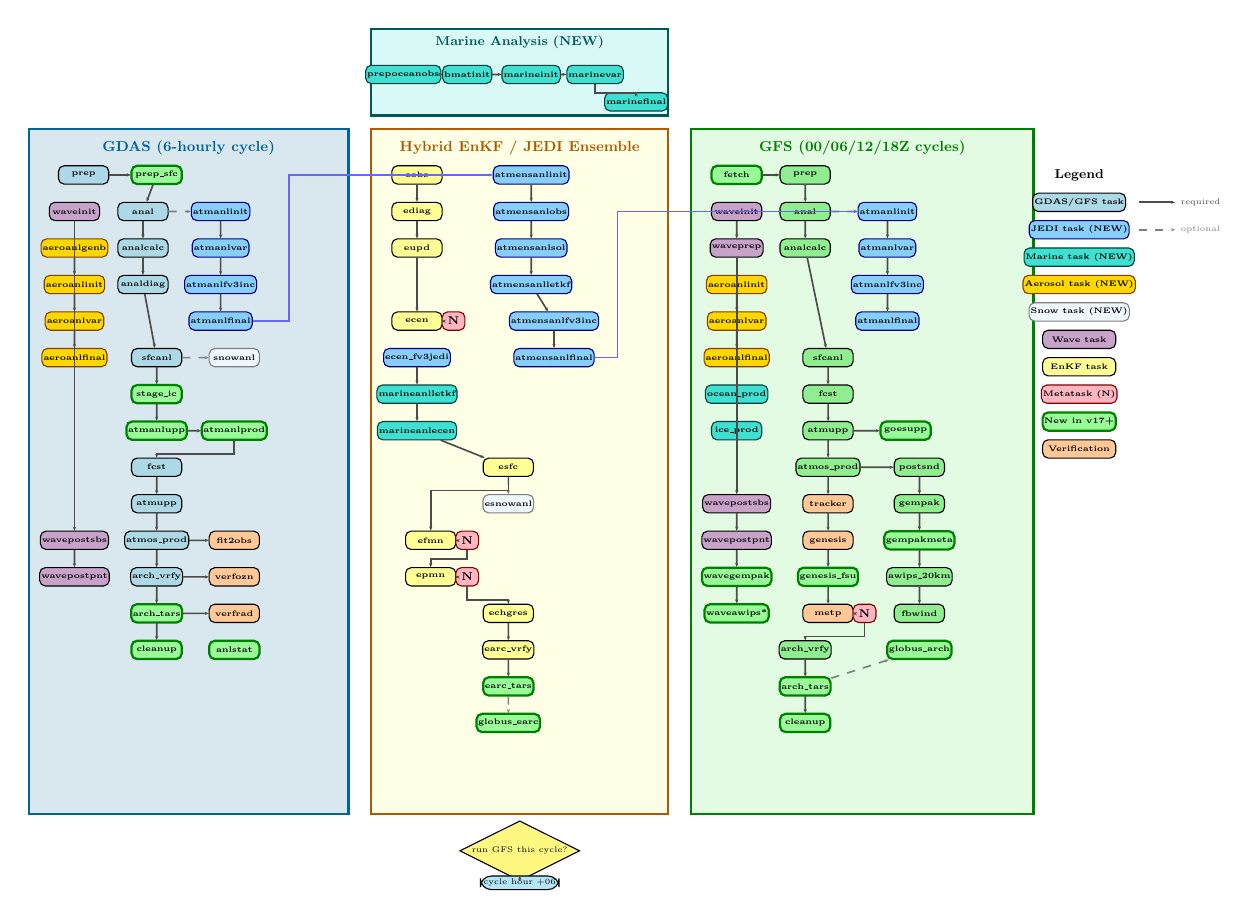
\begin{tikzpicture}[
    scale=0.58,
    transform shape,
    % Task styles - smaller boxes
    task/.style={rectangle, rounded corners=2pt, draw=black, minimum width=1.1cm, minimum height=0.4cm, font=\tiny\bfseries, align=center, inner sep=1pt},
    gdastask/.style={task, fill=GDASLight},
    gfstask/.style={task, fill=GFSGreen},
    enktask/.style={task, fill=EnKFYellow},
    wavetask/.style={task, fill=WavePurple},
    newtask/.style={task, fill=NewTask, draw=green!50!black, thick},
    jeditask/.style={task, fill=JEDIBlue, draw=blue!50!black},
    marinetask/.style={task, fill=MarineTeal, draw=teal!50!black},
    aerotask/.style={task, fill=AeroGold, draw=orange!50!black},
    snowtask/.style={task, fill=SnowWhite, draw=gray},
    metatask/.style={task, fill=EnKFPink, draw=red!50!black, minimum width=0.5cm},
    verifytask/.style={task, fill=VerifyOrange},
    % Arrow styles
    arrow/.style={-{Stealth[length=1.5pt]}, semithick, black!70},
    optarrow/.style={-{Stealth[length=1.5pt]}, semithick, dashed, black!50},
]

% ============================================================================
% GDAS REGION (Left side) - Contained box
% ============================================================================
\begin{scope}[local bounding box=gdas]
    \fill[GDASDark!15] (0,0) rectangle (7,-15);
    \draw[GDASDark, thick] (0,0) rectangle (7,-15);
    \node[font=\small\bfseries, color=GDASDark] at (3.5,-0.4) {GDAS (6-hourly cycle)};
    
    % Row 1: Pre-processing
    \node[gdastask] (gprep) at (1.2,-1) {prep};
    \node[newtask] (gprep_sfc) at (2.8,-1) {prep\_sfc};
    
    % Row 2: Wave + Analysis start
    \node[wavetask] (gwaveinit) at (1,-1.8) {waveinit};
    \node[gdastask] (ganal) at (2.5,-1.8) {anal};
    \node[jeditask] (gatmanlinit) at (4.2,-1.8) {atmanlinit};
    
    % Row 3: Aerosol + Analysis
    \node[aerotask] (gaeroanlgenb) at (1,-2.6) {aeroanlgenb};
    \node[gdastask] (ganalcalc) at (2.5,-2.6) {analcalc};
    \node[jeditask] (gatmanlvar) at (4.2,-2.6) {atmanlvar};
    
    % Row 4
    \node[aerotask] (gaeroanlinit) at (1,-3.4) {aeroanlinit};
    \node[gdastask] (ganaldiag) at (2.5,-3.4) {analdiag};
    \node[jeditask] (gatmanlfv3) at (4.2,-3.4) {atmanlfv3inc};
    
    % Row 5
    \node[aerotask] (gaeroanlvar) at (1,-4.2) {aeroanlvar};
    \node[jeditask] (gatmanlfinal) at (4.2,-4.2) {atmanlfinal};
    
    % Row 6
    \node[aerotask] (gaeroanlfinal) at (1,-5) {aeroanlfinal};
    \node[gdastask] (gsfcanl) at (2.8,-5) {sfcanl};
    \node[snowtask] (gsnowanl) at (4.5,-5) {snowanl};
    
    % Row 7: Staging
    \node[newtask] (gstage) at (2.8,-5.8) {stage\_ic};
    
    % Row 8: UPP
    \node[newtask] (gatmanlupp) at (2.8,-6.6) {atmanlupp};
    \node[newtask] (gatmanlprod) at (4.5,-6.6) {atmanlprod};
    
    % Row 9: Forecast
    \node[gdastask] (gfcst) at (2.8,-7.4) {fcst};
    
    % Row 10: Post
    \node[gdastask] (gatmupp) at (2.8,-8.2) {atmupp};
    
    % Row 11: Products + Wave
    \node[wavetask] (gwavepostsbs) at (1,-9) {wavepostsbs};
    \node[gdastask] (gatmosprod) at (2.8,-9) {atmos\_prod};
    \node[verifytask] (gfit2obs) at (4.5,-9) {fit2obs};
    
    % Row 12
    \node[wavetask] (gwavepostpnt) at (1,-9.8) {wavepostpnt};
    \node[gdastask] (garchvrfy) at (2.8,-9.8) {arch\_vrfy};
    \node[verifytask] (gverfozn) at (4.5,-9.8) {verfozn};
    
    % Row 13
    \node[newtask] (garchtars) at (2.8,-10.6) {arch\_tars};
    \node[verifytask] (gverfrad) at (4.5,-10.6) {verfrad};
    
    % Row 14
    \node[newtask] (gcleanup) at (2.8,-11.4) {cleanup};
    \node[newtask] (ganlstat) at (4.5,-11.4) {anlstat};
    
    % GDAS Arrows - main flow
    \draw[arrow] (gprep) -- (gprep_sfc);
    \draw[arrow] (gprep_sfc) -- (ganal);
    \draw[arrow] (ganal) -- (ganalcalc);
    \draw[arrow] (ganalcalc) -- (ganaldiag);
    \draw[optarrow] (ganal) -- (gatmanlinit);
    \draw[arrow] (gatmanlinit) -- (gatmanlvar);
    \draw[arrow] (gatmanlvar) -- (gatmanlfv3);
    \draw[arrow] (gatmanlfv3) -- (gatmanlfinal);
    \draw[arrow] (ganaldiag) -- (gsfcanl);
    \draw[optarrow] (gsfcanl) -- (gsnowanl);
    \draw[arrow] (gsfcanl) -- (gstage);
    \draw[arrow] (gstage) -- (gatmanlupp);
    \draw[arrow] (gatmanlupp) -- (gatmanlprod);
    \draw[arrow] (gatmanlprod.south) -- ++(0,-0.3) -| (gfcst.north);
    \draw[arrow] (gfcst) -- (gatmupp);
    \draw[arrow] (gatmupp) -- (gatmosprod);
    \draw[arrow] (gatmosprod) -- (garchvrfy);
    \draw[arrow] (garchvrfy) -- (garchtars);
    \draw[arrow] (garchtars) -- (gcleanup);
    % Wave flow
    \draw[arrow] (gwaveinit.south) -- ++(0,-5.8) -| (gwavepostsbs.north);
    \draw[arrow] (gwavepostsbs) -- (gwavepostpnt);
    % Aerosol flow
    \draw[arrow] (gaeroanlgenb) -- (gaeroanlinit);
    \draw[arrow] (gaeroanlinit) -- (gaeroanlvar);
    \draw[arrow] (gaeroanlvar) -- (gaeroanlfinal);
    % Verification
    \draw[arrow] (gatmosprod) -- (gfit2obs);
    \draw[arrow] (garchvrfy) -- (gverfozn);
    \draw[arrow] (garchtars) -- (gverfrad);
\end{scope}

% ============================================================================
% HYBRID EnKF / JEDI ENSEMBLE REGION (Center)
% ============================================================================
\begin{scope}[local bounding box=enkf]
    \fill[EnKFYellow!25] (7.5,0) rectangle (14,-15);
    \draw[orange!70!black, thick] (7.5,0) rectangle (14,-15);
    \node[font=\small\bfseries, color=orange!70!black] at (10.75,-0.4) {Hybrid EnKF / JEDI Ensemble};
    
    % GSI EnKF path (left) | JEDI path (right)
    \node[enktask] (eobs) at (8.5,-1) {eobs};
    \node[jeditask] (eatmensanlinit) at (11,-1) {atmensanlinit};
    
    \node[enktask] (ediag) at (8.5,-1.8) {ediag};
    \node[jeditask] (eobs_task) at (11,-1.8) {atmensanlobs};
    
    \node[enktask] (eupd) at (8.5,-2.6) {eupd};
    \node[jeditask] (esol_task) at (11,-2.6) {atmensanlsol};
    
    \node[jeditask] (eletkf) at (11,-3.4) {atmensanlletkf};
    
    % Centering
    \node[enktask] (ecen) at (8.5,-4.2) {ecen};
    \node[metatask] (ecenN) at (9.3,-4.2) {\scriptsize N};
    \node[jeditask] (efv3inc) at (11.5,-4.2) {atmensanlfv3inc};
    
    \node[jeditask] (ecen_fv3) at (8.5,-5) {ecen\_fv3jedi};
    \node[jeditask] (efinal) at (11.5,-5) {atmensanlfinal};
    
    % Marine ensemble
    \node[marinetask] (marineanlletkf) at (8.5,-5.8) {marineanlletkf};
    \node[marinetask] (marineanlecen) at (8.5,-6.6) {marineanlecen};
    
    % Surface and Snow
    \node[enktask] (esfc) at (10.5,-7.4) {esfc};
    \node[snowtask] (esnowanl) at (10.5,-8.2) {esnowanl};
    
    % Ensemble forecast
    \node[enktask] (efcsmn) at (8.8,-9) {efmn};
    \node[metatask] (efcsN) at (9.6,-9) {\scriptsize N};
    
    % Ensemble post
    \node[enktask] (eposmn) at (8.8,-9.8) {epmn};
    \node[metatask] (eposN) at (9.6,-9.8) {\scriptsize N};
    
    \node[enktask] (echgres) at (10.5,-10.6) {echgres};
    \node[enktask] (earcvrfy) at (10.5,-11.4) {earc\_vrfy};
    \node[newtask] (earctars) at (10.5,-12.2) {earc\_tars};
    \node[newtask] (globusearc) at (10.5,-13) {globus\_earc};
    
    % EnKF Arrows - GSI path
    \draw[arrow] (eobs) -- (ediag);
    \draw[arrow] (ediag) -- (eupd);
    \draw[arrow] (eupd) -- (ecen);
    \draw[arrow] (ecen) -- (ecenN);
    \draw[arrow] (ecen_fv3) -- (marineanlletkf);
    \draw[arrow] (marineanlletkf) -- (marineanlecen);
    
    % JEDI path
    \draw[arrow] (eatmensanlinit) -- (eobs_task);
    \draw[arrow] (eobs_task) -- (esol_task);
    \draw[arrow] (esol_task) -- (eletkf);
    \draw[arrow] (eletkf) -- (efv3inc);
    \draw[arrow] (efv3inc) -- (efinal);
    
    % Merge and continue
    \draw[arrow] (marineanlecen) -- (esfc);
    \draw[optarrow] (esfc) -- (esnowanl);
    \draw[arrow] (esfc.south) -- ++(0,-0.3) -| (efcsmn.north);
    \draw[arrow] (efcsmn) -- (efcsN);
    \draw[arrow] (efcsN.south) -- ++(0,-0.2) -| (eposmn.north);
    \draw[arrow] (eposmn) -- (eposN);
    \draw[arrow] (eposN.south) -- ++(0,-0.3) -| (echgres.north);
    \draw[arrow] (echgres) -- (earcvrfy);
    \draw[arrow] (earcvrfy) -- (earctars);
    \draw[optarrow] (earctars) -- (globusearc);
\end{scope}

% ============================================================================
% GFS REGION (Right side)
% ============================================================================
\begin{scope}[local bounding box=gfs]
    \fill[GFSGreen!25] (14.5,0) rectangle (22,-15);
    \draw[green!50!black, thick] (14.5,0) rectangle (22,-15);
    \node[font=\small\bfseries, color=green!50!black] at (18.25,-0.4) {GFS (00/06/12/18Z cycles)};
    
    % Row 1: Fetch + Prep
    \node[newtask] (fetch) at (15.5,-1) {fetch};
    \node[gfstask] (fprep) at (17,-1) {prep};
    
    % Row 2: Wave + Analysis
    \node[wavetask] (fwaveinit) at (15.5,-1.8) {waveinit};
    \node[gfstask] (fanal) at (17,-1.8) {anal};
    \node[jeditask] (fatmanlinit) at (18.8,-1.8) {atmanlinit};
    
    % Row 3
    \node[wavetask] (fwaveprep) at (15.5,-2.6) {waveprep};
    \node[gfstask] (fanalcalc) at (17,-2.6) {analcalc};
    \node[jeditask] (fatmanlvar) at (18.8,-2.6) {atmanlvar};
    
    % Row 4
    \node[aerotask] (faeroanlinit) at (15.5,-3.4) {aeroanlinit};
    \node[jeditask] (fatmanlfv3) at (18.8,-3.4) {atmanlfv3inc};
    
    % Row 5
    \node[aerotask] (faeroanlvar) at (15.5,-4.2) {aeroanlvar};
    \node[jeditask] (fatmanlfinal) at (18.8,-4.2) {atmanlfinal};
    
    % Row 6
    \node[aerotask] (faeroanlfinal) at (15.5,-5) {aeroanlfinal};
    \node[gfstask] (fsfcanl) at (17.5,-5) {sfcanl};
    
    % Row 7: Ocean products + Forecast
    \node[marinetask] (foceanprod) at (15.5,-5.8) {ocean\_prod};
    \node[gfstask] (ffcst) at (17.5,-5.8) {fcst};
    
    % Row 8
    \node[marinetask] (ficeprod) at (15.5,-6.6) {ice\_prod};
    \node[gfstask] (fatmupp) at (17.5,-6.6) {atmupp};
    \node[newtask] (fgoesupp) at (19.2,-6.6) {goesupp};
    
    % Row 9
    \node[gfstask] (fatmosprod) at (17.5,-7.4) {atmos\_prod};
    \node[gfstask] (fpostsnd) at (19.5,-7.4) {postsnd};
    
    % Row 10: Wave post + Tracking
    \node[wavetask] (fwavepostsbs) at (15.5,-8.2) {wavepostsbs};
    \node[verifytask] (ftracker) at (17.5,-8.2) {tracker};
    \node[gfstask] (fgempak) at (19.5,-8.2) {gempak};
    
    % Row 11
    \node[wavetask] (fwavepostpnt) at (15.5,-9) {wavepostpnt};
    \node[verifytask] (fgenesis) at (17.5,-9) {genesis};
    \node[newtask] (fgempakmeta) at (19.5,-9) {gempakmeta};
    
    % Row 12
    \node[newtask] (fwavegempak) at (15.5,-9.8) {wavegempak};
    \node[newtask] (fgenesisfsu) at (17.5,-9.8) {genesis\_fsu};
    \node[gfstask] (fawips) at (19.5,-9.8) {awips\_20km};
    
    % Row 13
    \node[newtask] (fwaveawips) at (15.5,-10.6) {waveawips*};
    \node[verifytask] (fmetp) at (17.5,-10.6) {metp};
    \node[metatask] (fmetpN) at (18.3,-10.6) {\scriptsize N};
    \node[gfstask] (ffbwind) at (19.5,-10.6) {fbwind};
    
    % Row 14: Archive
    \node[gfstask] (farchvrfy) at (17,-11.4) {arch\_vrfy};
    \node[newtask] (fglobus) at (19.5,-11.4) {globus\_arch};
    
    % Row 15
    \node[newtask] (farchtars) at (17,-12.2) {arch\_tars};
    
    % Row 16
    \node[newtask] (fcleanup) at (17,-13) {cleanup};
    
    % GFS Arrows - main flow
    \draw[arrow] (fetch) -- (fprep);
    \draw[arrow] (fprep) -- (fanal);
    \draw[arrow] (fanal) -- (fanalcalc);
    \draw[optarrow] (fanal) -- (fatmanlinit);
    \draw[arrow] (fatmanlinit) -- (fatmanlvar);
    \draw[arrow] (fatmanlvar) -- (fatmanlfv3);
    \draw[arrow] (fatmanlfv3) -- (fatmanlfinal);
    \draw[arrow] (fanalcalc) -- (fsfcanl);
    \draw[arrow] (fsfcanl) -- (ffcst);
    \draw[arrow] (ffcst) -- (fatmupp);
    \draw[arrow] (fatmupp) -- (fatmosprod);
    \draw[arrow] (fatmupp) -- (fgoesupp);
    \draw[arrow] (fatmosprod) -- (ftracker);
    \draw[arrow] (ftracker) -- (fgenesis);
    \draw[arrow] (fgenesis) -- (fgenesisfsu);
    \draw[arrow] (fgenesisfsu) -- (fmetp);
    \draw[arrow] (farchvrfy) -- (farchtars);
    \draw[arrow] (farchtars) -- (fcleanup);
    \draw[optarrow] (farchtars) -- (fglobus);
    % Wave flow
    \draw[arrow] (fwaveinit) -- (fwaveprep);
    \draw[arrow] (fwaveprep.south) -- ++(0,-4.2) -| (fwavepostsbs.north);
    \draw[arrow] (fwavepostsbs) -- (fwavepostpnt);
    \draw[arrow] (fwavepostpnt) -- (fwavegempak);
    \draw[arrow] (fwavegempak) -- (fwaveawips);
    % Aerosol flow
    \draw[arrow] (faeroanlinit) -- (faeroanlvar);
    \draw[arrow] (faeroanlvar) -- (faeroanlfinal);
    % Products flow
    \draw[arrow] (fatmosprod) -- (fpostsnd);
    \draw[arrow] (fpostsnd) -- (fgempak);
    \draw[arrow] (fgempak) -- (fgempakmeta);
    \draw[arrow] (fgempakmeta) -- (fawips);
    \draw[arrow] (fawips) -- (ffbwind);
    % Archive from products
    \draw[arrow] (fmetp) -- (fmetpN);
    \draw[arrow] (fmetpN.south) -- ++(0,-0.3) -| (farchvrfy.north);
\end{scope}

% ============================================================================
% MARINE ANALYSIS SYSTEM (NEW - Top banner)
% ============================================================================
\begin{scope}[local bounding box=marine]
    \fill[MarineTeal!20] (7.5,2.2) rectangle (14,0.3);
    \draw[teal!70!black, thick] (7.5,2.2) rectangle (14,0.3);
    \node[font=\footnotesize\bfseries, color=teal!70!black] at (10.75,1.9) {Marine Analysis (NEW)};
    
    \node[marinetask, minimum width=0.9cm] (prepoceanobs) at (8.2,1.2) {prepoceanobs};
    \node[marinetask, minimum width=0.9cm] (marinebmatinit) at (9.6,1.2) {bmatinit};
    \node[marinetask, minimum width=0.9cm] (marineanlinit) at (11,1.2) {marineinit};
    \node[marinetask, minimum width=0.9cm] (marineanlvar) at (12.4,1.2) {marinevar};
    \node[marinetask, minimum width=0.9cm] (marineanlfinal) at (13.3,0.6) {marinefinal};
    
    % Marine arrows
    \draw[arrow] (prepoceanobs) -- (marinebmatinit);
    \draw[arrow] (marinebmatinit) -- (marineanlinit);
    \draw[arrow] (marineanlinit) -- (marineanlvar);
    \draw[arrow] (marineanlvar.south) -- ++(0,-0.2) -| (marineanlfinal.north);
\end{scope}

% ============================================================================
% CROSS-REGION CONNECTIONS
% ============================================================================
% GDAS -> EnKF (analysis to ensemble)
\draw[arrow, blue!60] (gatmanlfinal.east) -- ++(0.8,0) |- (eatmensanlinit.west);
% EnKF -> GFS (ensemble to forecast)  
\draw[arrow, blue!60] (efinal.east) -- ++(0.5,0) |- (fatmanlinit.west);

% ============================================================================
% CYCLE LOGIC (Bottom Center)
% ============================================================================
\node[draw, diamond, fill=yellow!50, aspect=2, font=\tiny, inner sep=1pt] (cyclelogic) at (10.75,-15.8) {run GFS this cycle?};
\node[draw, rectangle, rounded corners, fill=cyan!30, font=\tiny, inner sep=2pt] (cyclehour) at (10.75,-16.5) {cycle hour +06};
\draw[arrow] (cyclelogic) -- (cyclehour);

% ============================================================================
% LEGEND (Far right, outside regions)
% ============================================================================
\begin{scope}[xshift=23cm, yshift=-3cm]
    \node[font=\footnotesize\bfseries] at (0,2) {Legend};
    
    \node[gdastask, minimum width=1.6cm] (leg1) at (0,1.4) {GDAS/GFS task};
    \node[jeditask, minimum width=1.6cm] (leg2) at (0,0.8) {JEDI task (NEW)};
    \node[marinetask, minimum width=1.6cm] (leg3) at (0,0.2) {Marine task (NEW)};
    \node[aerotask, minimum width=1.6cm] (leg4) at (0,-0.4) {Aerosol task (NEW)};
    \node[snowtask, minimum width=1.6cm] (leg5) at (0,-1.0) {Snow task (NEW)};
    \node[wavetask, minimum width=1.6cm] (leg6) at (0,-1.6) {Wave task};
    \node[enktask, minimum width=1.6cm] (leg7) at (0,-2.2) {EnKF task};
    \node[metatask, minimum width=1.6cm] (leg8) at (0,-2.8) {Metatask (N)};
    \node[newtask, minimum width=1.6cm] (leg9) at (0,-3.4) {New in v17+};
    \node[verifytask, minimum width=1.6cm] (leg10) at (0,-4.0) {Verification};
    
    \draw[arrow] (1.3,1.4) -- (2.1,1.4) node[right, font=\tiny] {required};
    \draw[optarrow] (1.3,0.8) -- (2.1,0.8) node[right, font=\tiny] {optional};
\end{scope}

\end{tikzpicture}
\caption{Global Model Parallel Sequencing v17+ --- Updated from v16 with JEDI, Marine, and Aerosol Analysis Systems}
\label{fig:workflow-v17}
\end{figure}

\newpage

% ============================================================================
% CHANGES FROM v16 TABLE
% ============================================================================

\section*{Changes from v16 to v17+}

\begin{table}[H]
\centering
\caption{New Tasks Added Since v16}
\small
\begin{tabular}{@{}llp{8cm}@{}}
\toprule
\textbf{Category} & \textbf{Task(s)} & \textbf{Description} \\
\midrule
\multicolumn{3}{l}{\textbf{JEDI Atmospheric Analysis (replaces GSI optionally)}} \\
& atmanlinit & Initialize JEDI atm analysis \\
& atmanlvar & JEDI variational solver \\
& atmanlfv3inc & Generate FV3 increment \\
& atmanlfinal & Finalize JEDI analysis \\
& analcalc\_fv3jedi & FV3JEDI analysis calculation \\
\midrule
\multicolumn{3}{l}{\textbf{JEDI Ensemble Analysis}} \\
& atmensanlinit & Initialize ensemble analysis \\
& atmensanlobs & Ensemble observation processing \\
& atmensanlsol & Ensemble solver \\
& atmensanlletkf & LETKF solver \\
& atmensanlfv3inc & Ensemble FV3 increment \\
& atmensanlfinal & Finalize ensemble analysis \\
& ecen\_fv3jedi & FV3JEDI ensemble centering \\
\midrule
\multicolumn{3}{l}{\textbf{Marine Analysis System (SOCA)}} \\
& prepoceanobs & Prepare ocean observations \\
& marinebmatinit & Initialize marine B-matrix \\
& marinebmat & Compute marine B-matrix \\
& marineanlinit & Initialize marine analysis \\
& marineanlvar & Marine variational analysis \\
& marineanlchkpt & Marine analysis checkpoint \\
& marineanlfinal & Finalize marine analysis \\
& marineanlletkf & Marine LETKF (ensemble) \\
& marineanlecen & Marine ensemble centering \\
\midrule
\multicolumn{3}{l}{\textbf{Aerosol Analysis}} \\
& aeroanlgenb & Generate aerosol B-matrix \\
& aeroanlinit & Initialize aerosol analysis \\
& aeroanlvar & Aerosol variational analysis \\
& aeroanlfinal & Finalize aerosol analysis \\
& aerosol\_init & Aerosol initialization (fcst-only) \\
\midrule
\multicolumn{3}{l}{\textbf{Snow Analysis}} \\
& snowanl & JEDI snow analysis \\
& esnowanl & Ensemble snow analysis \\
\midrule
\multicolumn{3}{l}{\textbf{New Products}} \\
& ocean\_prod & Ocean products \\
& ice\_prod & Ice products \\
& atmanlupp & Analysis UPP \\
& atmanlprod & Analysis products \\
& goesupp & GOES post-processing \\
\midrule
\multicolumn{3}{l}{\textbf{Staging/Fetching}} \\
& fetch & Fetch data from HPSS \\
& stage\_ic & Stage initial conditions \\
\midrule
\multicolumn{3}{l}{\textbf{Wave Enhancements}} \\
& wavegempak & Wave GEMPAK products \\
& waveawipsbulls & Wave AWIPS bulletins \\
& waveawipsgridded & Wave AWIPS gridded \\
\midrule
\multicolumn{3}{l}{\textbf{Verification/Tracking}} \\
& genesis\_fsu & FSU genesis tracker \\
& anlstat & Analysis statistics \\
\midrule
\multicolumn{3}{l}{\textbf{Archive System Modernization}} \\
& arch\_vrfy & Archive verification \\
& arch\_tars & Archive tarballs \\
& earc\_vrfy & Ensemble archive verification \\
& earc\_tars & Ensemble archive tarballs \\
& globus\_arch & Globus archive transfer \\
& globus\_earc & Globus ensemble archive \\
& cleanup & Explicit cleanup task \\
\bottomrule
\end{tabular}
\end{table}

\begin{table}[H]
\centering
\caption{Tasks Removed or Renamed from v16}
\small
\begin{tabular}{@{}lll@{}}
\toprule
\textbf{v16 Task} & \textbf{Status} & \textbf{Notes} \\
\midrule
gldas & Removed & GLDAS land DA deprecated \\
post/postN & Renamed & Now atmupp + atmos\_prod \\
arch & Split & Now arch\_vrfy + arch\_tars \\
earc/eamn & Renamed & Now earc\_vrfy + earc\_tars \\
vrfy & Expanded & Multiple verification tasks \\
\bottomrule
\end{tabular}
\end{table}

\section*{New Application Types Since v16}

\begin{itemize}
    \item \textbf{SFS} (Subseasonal Forecast System) --- New forecast-only application
    \item \textbf{GCAFS} (Global Climate and Air quality Forecasting System) --- Cycled and forecast-only modes
    \item \textbf{GEFS} (Global Ensemble Forecast System) --- Enhanced with 21 tasks
\end{itemize}

\section*{Task Count Comparison}

\begin{table}[H]
\centering
\begin{tabular}{@{}lrr@{}}
\toprule
\textbf{Metric} & \textbf{v16} & \textbf{v17+} \\
\midrule
Total J-Jobs & $\sim$50 & 89 \\
GFS Tasks (gfs\_tasks.py) & $\sim$35 & 89 methods \\
GEFS Tasks (gefs\_tasks.py) & --- & 21 \\
SFS Tasks (sfs\_tasks.py) & --- & 18 \\
Application Types & 2 & 6 \\
\bottomrule
\end{tabular}
\end{table}

\end{document}
